\documentclass[a4paper, 12pt]{article}

\renewcommand{\familydefault}{\sfdefault}

\usepackage[french, english]{babel}
\usepackage{amsmath}
\usepackage{amssymb}
\usepackage{parskip}
\usepackage{graphicx}
\graphicspath{ {./images/} }
\usepackage{capt-of}
\usepackage{makecell}

\setlength{\arrayrulewidth}{0.3mm}
\setlength{\tabcolsep}{18pt}

\begin{document}
\title{\Large{\textbf{Machine Learning Algebra}}}
\author{By Matthieu Lagarde}
\date{April 9, 2022}

\maketitle

\setcounter{page}{2}

\newpage
\section{Multivariate linear regression}
\subsection{Notations}

Let $m$ be the number of examples or observations in our training set. Let $n$ be the number of features or explanatory variables observed for each example of the training set. Let $x_j^{(i)}$ be the value of feature $j$ for example $i$. Let $y^{(i)}$ be the output value for example $i$.

\begin{equation}
y = \begin{pmatrix}  y^{(1)} \\ y^{(2)} \\ ... \\ y^{(m)} \end{pmatrix} \in \mathbb{R}^{m} 
\end{equation}

\noindent
$y$ is called the output vector. It contains the output values of the training set.

\begin{equation}
X = \begin{pmatrix} 1 & x_1^{(1)} & x_2^{(1)} & ... & x_n^{(1)} \\  1 & x_1^{(2)} & x_2^{(2)} & ... & x_n^{(2)} \\ ... & ... & ... & ... \\ 1 & x_1^{(m)} & x_2^{(m)} & ... & x_n^{(m)} \end{pmatrix} \in \mathbb{R}^{m\times(n+1)} 
\end{equation}

\noindent
$X$ is called the data matrix. If we ignore the first column of $1$, each row of matrix $X$ is one example of the training set and each column of the matrix $X$ is the values observed for one feature in the training set.

\begin{equation}
\theta = \begin{pmatrix}  \theta_0 \\ \theta_1 \\ ... \\ \theta_n \end{pmatrix} \in \mathbb{R}^{(n+1)} 
\end{equation}

$\theta$ is the vector of parameters.

\subsection{Hypothesis}

We assume that there is a linear relationship between the features and the output. Note that the relationship is linear in $\theta$ but the features themselves can be non linear transformations of the initial features such as quadratic terms or interaction terms.

\noindent
The unvectorized form of the hypothesis for a given example $i$ is:

\begin{equation}
h_{\theta}(x^{(i)}) = \sum_{j=0}^{n} \theta_j * x_j^{(i)} \in \mathbb{R} \; with \;  x_0^{(i)}=1
\end{equation}

\noindent
The vectorized form of the hypothesis can be written as follows:

\begin{equation}
h_{\theta}(X) = X\theta \in \mathbb{R}^{m} 
\end{equation}

\noindent
For a single example, we can also write the vectorized form of the hypothesis:

\begin{align*} 
& x^{(i)} = \begin{pmatrix} 1 \\ x_1^{(i)} \\ ... \\ x_n^{(i)} \end{pmatrix}  \in \mathbb{R}^{(n+1)}  \\
& \\
& h_{\theta}(x^{(i)})  = x^{(i)^{\top}}\theta \in \mathbb{R}
\end{align*}

\subsection{Cost function}

\noindent
The unvectorized form of the cost function is:

\begin{align*}
& J(\theta) = \frac{1}{2m} * \sum_{i=1}^{m} (h_{\theta}(x^{(i)}) - y^{(i)})^{2} \in \mathbb{R} \\
& where \; x^{(i)} \in \mathbb{R}^{(n+1)} \; and \\
& where \; y^{(i)} \in \mathbb{R}
\end{align*}

\noindent
The vectorized form of the cost function is:

\begin{equation}
J(\theta) = \frac{1}{2m} * (X\theta - y)^{\top}(X\theta - y) \in \mathbb{R}
\end{equation}

\subsection{Normal equation}

$J(\theta)$ is convex so any local minimum is  a global minimum. We thus know that $\theta^{*}$ obeys the following equation:

\begin{align*}
\nabla J(\theta^{*}) = 0_{(n+1)}
\end{align*}

Let recall a property of matrix differentiation. Let $\alpha$ be a scalar equal to $y^{\top}x$ where $y$ and $x$ be two column vectors of $\mathbb{R}^m$ that are respectively a function of another column vector $z$ of $\mathbb{R}^n$. We have:

\begin{align*}
& \alpha = y^{\top}x \\
& \\
& \frac{\partial \alpha}{\partial z}= {\frac{\partial y}{\partial z}}^{\top}x + {\frac{\partial x}{\partial z}}^{\top}y \in \mathbb{R}^n
\end{align*}

Using this property, we have:

\begin{align*}
& 1/2m*2*{\frac{\partial (X\theta^* - y)}{\partial \theta}}^{\top}(X\theta^* - y) = 0_{(n+1)} \\
& \iff 1/m*X^{\top}(X\theta^* - y) = 0_{(n+1)} \\
& \iff X^{\top}X\theta^* - X^{\top}y = 0_{(n+1)} \\
& \boxed{\iff \theta^* = {(X^{\top}X)}^{-1}X^{\top}y \in \mathbb{R}^{(n+1)}}
\end{align*}

\subsection{Gradient descent}

If necessary, here is the vectorized implementation of gradient descent. Denoting $\alpha$ the learning rate:

\begin{equation}
\theta := \theta - \frac{\alpha}{m} * X^{\top}(X\theta- y) \in \mathbb{R}^{(n+1)}
\end{equation}

\subsection{Regularized cost function}

Denoting $\lambda$  the regularization parameter, the unvectorized form of the cost function can be written as:

\begin{align*}
& J(\theta) = \frac{1}{2m} * \sum_{i=1}^{m} (h_{\theta}(x^{(i)}) - y^{(i)})^{2} + \frac{\lambda}{2m}*\sum_{j=1}^{n} \theta_j^{2}  \in \mathbb{R} \\
& where \; x^{(i)} \in \mathbb{R}^{(n+1)} \; and \\
& where \; y^{(i)} \in \mathbb{R}
\end{align*}

Be careful, in the regularization part of the expression (the second sum), the $j$ index goes from $1$ to $n$ and NOT from $0$ to $n$. Indeed, by convention, we do not regularize $\theta_0$.

The vectorized form of the regularized cost function is thus:

\begin{align*}
& J(\theta) =  \frac{1}{2m} * (X\theta - y)^{\top}(X\theta - y) + \frac{\lambda}{2m}*\theta_{r}^{\top}\theta_{r} \\
& where \; \theta_{r} =  \begin{pmatrix}  \theta_1 \\ ... \\ \theta_n \end{pmatrix} \in \mathbb{R}^{n} 
\end{align*}

\subsection{Regularized normal equation}

The vectorized form of the regularized normal equation is:

\begin{align*}
& \theta^* = {(X^{\top}X + \lambda*M)}^{-1}X^{\top}y \in \mathbb{R}^{(n+1)} \\
& where \; M = \begin{pmatrix}0 & 0 & 0 & ... & 0 \\ 0 & 1 & 0 & ... & 0 \\ ... & ... & ... & ... & ... \\ 0 & 0 & ... & 1 & 0 \\ 0 & 0 & ... & 0 & 1\end{pmatrix} \in \mathbb{R}^{(n+1)\times(n+1)}
\end{align*}

\subsection{Regularized gradient descent}

Let compute the gradient of $J(\theta)$ when it is regularized. There are two cases, one for the partial derivative with respect to $\theta_0$ and one for the partial derivatives with respect to $\theta_j$:

\begin{align*}
& \frac{\partial J(\theta)}{\partial \theta_0} = {\left[ \frac{1}{m}*X^{\top}(X\theta-y) \right]}_{1} \; i.e. \; 1st \; element \; of \; previous \; gradient \\
& \\
& \frac{\partial J(\theta)}{\partial \theta_j} = {\left[ \frac{1}{m}*X^{\top}(X\theta-y) + \frac{\lambda}{m} * \theta \right]}_{j+1} \; for \; j \in \{1, 2, ..., n\} 
\end{align*}

\section{Logistic regression}

\subsection{Sigmoid function}

Let introduce the sigmoid function:

\begin{equation}
g \; : \; x \in \mathbb{R} \longrightarrow  \frac{1}{1+e^{-x}} \in \left] 0, 1 \right[
\end{equation}

The interesting properties of the sigmoid function are:
\begin{itemize}
\item It is defined over $\mathbb{R}$.
\item It is increasing. 
\item $g(0) = \frac{1}{2}$.
\item It is converging to 0 in $-\infty$ and to 1 in $+\infty$.
\item It is convex over $\left] -\infty, 0 \right]$ and concave over $\left[ 0, +\infty \right[$.
\item It means that (0, 0.5) is an inflection point of $g$.
\item $g(-4) = 0.02 $ and $g(4) = 0.98 $
\end{itemize}

\begin{center}
  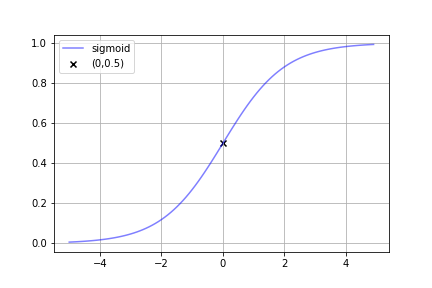
\includegraphics[scale=0.7]{sigmoid}
  \captionof{figure}{Graph of the sigmoid function}
  \label{fig:sigmoid}
\end{center}

\subsection{Hypothesis}

\noindent
The unvectorized form of the hypothesis for a given example $i$ is:

\begin{align*}
& h_{\theta}(x^{(i)}) = g \left( \sum_{j=0}^{n} \theta_j * x_j^{(i)}  \right) \in \left]0, 1\right[  \\
& \\
& where \; g \; is \; the \; sigmoid \; function.
\end{align*}

The hypothesis can be interpreted as the probability that a new observation belongs to the positive class i.e. that $y=1$ given the value of its features i.e. given $x$, parameterized by $\theta$. In other words:

\begin{equation}
h_{\theta}(x) = P\left(y=1|x;\theta \right)
\end{equation}

We then introduce the following decision rule:

\begin{equation}
y = 
\begin{cases}
1 & \text{if } h_{\theta}(x) \geq 0.5 \\
0 & \text{if } h_{\theta}(x) < 0.5
\end{cases}
\end{equation}

Finally, the vectorized form of the hypothesis can be written as follows:

\begin{align*}
& h_{\theta}(X) = g\left(X\theta\right) \in \left]0, 1\right[^{m} \\
& \text{where g is the sigmoid function applied element-wise}
\end{align*}

\subsection{Cost function}

Before introducing the cost function, let study two functions:

\begin{align*}
& v \; : \; x \in \left] 0, 1 \right[ \longrightarrow  -ln(x) \in \left[0, +\infty\right[ \\
& \\
& w \; : \; x \in \left] 0, 1 \right[ \longrightarrow  -ln(1-x) \in \left[0, +\infty\right[ \\
\end{align*}

Function $v$ has the following properties on the interval $\left] 0, 1 \right[$ :

\begin{itemize}
\item It is decreasing.
\item It converges to $+\infty$ in 0.
\item $v(1)=0$.
\end{itemize}

Function $w$ has the following properties on the interval $\left] 0, 1 \right[$ :

\begin{itemize}
\item It is increasing.
\item It converges to $+\infty$ in 1.
\item $w(0)=0$.
\end{itemize}

Here is the graph of $v$ and $w$ on the interval $\left] 0, 1 \right[$ :

\begin{center}
  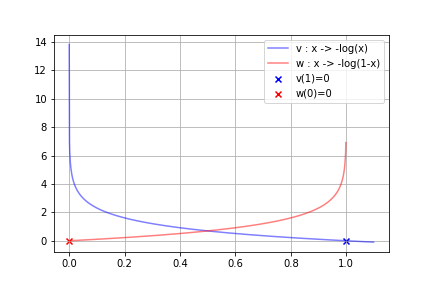
\includegraphics[scale=0.7]{vw}
  \captionof{figure}{Graph of $v$ and $w$}
  \label{fig:vw}
\end{center}

Now we introduce the following cost function:

\begin{align*}
& J(\theta) = \frac{1}{m} * \sum_{i=1}^{m} Cost\left(h_{\theta}\left(x^{(i)}\right), y^{(i)}\right) \in \mathbb{R} \\
& \text{where} \\
& Cost\left(h_{\theta}\left(x^{(i)}\right), y^{(i)}\right)  =
\begin{cases}
-ln\left(h_{\theta}\left(x^{(i)}\right)\right) & \text{ if } y^{(i)}=1 \\
-ln\left(1-h_{\theta}\left(x^{(i)}\right)\right) & \text{ if } y^{(i)}=0
\end{cases}
\end{align*}

Given that $y \in \{0, 1\}$, the cost function can be rewritten as:

\begin{equation}
J(\theta) = \frac{1}{m} * \sum_{i=1}^{m} \left[  \left(y^{(i)} * -ln\left(h_{\theta}\left(x^{(i)}\right)\right)\right) + \left( (1-y^{(i)}) * -ln\left(1-h_{\theta}\left(x^{(i)}\right)\right)  \right) \right] \in \mathbb{R}
\end{equation}

We can also write the vectorized form of the cost function as follows:

\begin{align*}
& J(\theta) = -\frac{1}{m} * \left[y^{\top} ln(h_{\theta}(X)) + (1-y)^{\top}ln(1-h_{\theta}(X)) \right] \in \mathbb{R} \\
& \\
& \text{where } ln \text{ is applied element-wise} 
\end{align*}

\subsection{Gradient descent}

The unvectorized form of the gradient of the cost function can be written as:

\begin{equation}
\frac{\partial J(\theta)}{\partial \theta_{k}} = \frac{1}{m} * \sum_{i=1}^{m} \left( \frac{1}{1+exp(-\sum_{j=0}^{n} x_{j}^{(i)}*\theta_{j})} - y^{(i)} \right) * x_{k}^{(i)} \in \mathbb{R}
\end{equation}

The vectorized form of the gradient of the cost function can be written as:

\begin{align*}
& \nabla J(\theta) = \frac{1}{m} * X^{\top}\left( h_{\theta}(X)-y \right) \in \mathbb{R}^{n+1} \\
& \\
& \text{where } h_{\theta}(X) \in \left]0, 1 \right[^{m} \\
\end{align*}

Denoting $\alpha$ the learning rate, a vectorized implementation of the gradient descent can thus be written as:

\begin{align*}
& \theta := \theta - \frac{\alpha}{m} *X^{\top}\left( h_{\theta}(X)-y \right) \in \mathbb{R}^{n+1} \\
& \\
& \text{where } h_{\theta}(X) = g(X\theta ) \in \left] 0, 1 \right[^{m} \\
& \\
& \text{and g is the sigmoid function applied element-wise}
\end{align*}

\subsection{Regularization}

The regularized cost function can be written as:

\begin{align*}
& J(\theta) = -\frac{1}{m} * \left[y^{\top} ln(h_{\theta}(X)) + (1-y)^{\top}ln(1-h_{\theta}(X)) \right] +\frac{\lambda}{2m}*\theta_{r}^{\top}\theta_{r}  \in \mathbb{R} \\
& \\
& \text{where } ln \text{ is applied element-wise} 
\end{align*}

The regularized gradient can be written as:

\begin{align*}
& {\left [ \widetilde{\nabla J(\theta)} \right]}_{1} = {\left [ \nabla J(\theta) \right]}_{1} \text{for } \partial \theta_{0} \text{ i.e. the first element of the regularized gradient} \\
& {\left [ \widetilde{\nabla J(\theta)} \right]}_{j} = {\left [ \nabla J(\theta) + \frac{\lambda}{m}*\theta \right]}_{j} \text{where } j \in \{2, 3, ..., n\}
\end{align*}

\section{Neural network classifier}
\subsection{Notations}

Let consider the following neural network:

\begin{center}
  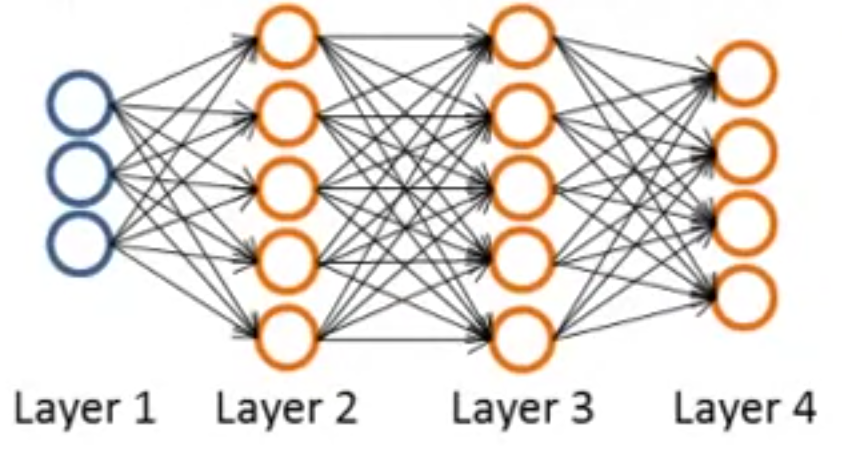
\includegraphics{neural}
  \captionof{figure}{Example of neural network}
  \label{fig:neural}
\end{center}

We assume that we face a multi-class classification where we want to predict whether an observation belongs to one of $K$ possible classes. We denote $L$ the total number of layers in the network.

By convention, the input layer is not counted as a true layer. So in this example, we are facing a 3-layer neural network. The first layer is called the input layer and is not counted in the total, it is indexed as layer 0. The last layer is called the output layer, it is indexed as layer 3 in this example.

Intermediate layers are called hidden layers. Here, there are 2 hidden layers. We denote $n_{h}^{[l]}$ the number of units in layer $l$, not counting the bias unit. In the example, we thus have:

\begin{itemize}
\item $n_{h}^{[0]} = 3$ which is $n_x$, the number of input features.
\item $n_{h}^{[1]} = 5$.
\item $n_{h}^{[2]} = 5$.
\item $n_{h}^{[3]} = 4$ which is $K$ or $n_y$ or $n_{h}^{[L]}$, the number of classes.
\end{itemize}

We assume that a bias unit is added as an input to any layer. We denote $m$ the total number of examples in our training set.

We are going to change a bit our notations for solving neural networks as it will be more convenient. The data matrix $X$ is gonna be transposed i.e. we are going to stack horizontally each training example.

$X = \begin{pmatrix} x^{(1)} & x^{(2)} & ... & x^{(m)} \end{pmatrix} \in \mathbb{R}^{n_{x}\times m}$

We are doing the same for the output label matrix:

$Y = \begin{pmatrix} y^{(1)} & y^{(2)} & ... & y^{(m)} \end{pmatrix} \in \mathbb{R}^{n_{y}\times m}$

Both for $X$ and $Y$, the number of rows is equal to the number of features (resp. classes) and the number of columns is equal to the number of training examples. One column corresponds to one training example. 

Finally, we denote $W^{[l]}$ the weight matrix required to go from layer $(l-1)$ to layer $l$. This matrix is in the space $\mathbb{R}^{n_h^{[l]} \times n_h^{[l-1]}}$ since it maps vectors of dimension $n_h^{[l-1]}$  into vectors of dimension $n_h^{[l]}$. The number of rows correspond to the number of units in the next layer while the number of columns correspond to the number of units in the previous layer!

Note that in this example, there are 3 matrices of parameters to estimate : $W^{[1]}$, $W^{[2]}$ and $W^{[3]}$. It requires to estimate $5*3 + 5*5 + 4*5 = 15 + 25 + 20 = 60$ weights, without counting the weights associated to the biais units. 

Finally, the i-th row of matrix $W^{[l]}$ corresponds to the weights used to compute the i-th activation unit of layer $l$.

We also introduce the bias vectors $b^{[l]}$ of layer $l$:

$b^{[l]} \in \mathbb{R}^{n_h^{[l]}}$

There is one weight for each activation unit of layer $l$.

\subsection{Forward propagation}

Given the data matrix $X$ and weights $W^{[1]}, b^{[1]}, ..., W^{[L]}, b^{[L]}$ that have been initialized randomly, we can compute the hypothesis i.e. the matrix $\hat{Y}$ giving the probability that each training example $x^{(i)}$ belongs to each class.

\begin{align*}
& X = A^{[0]} \in n_x \times m  \\
& \text{For } l \in [1, ..., L] \\
&  Z^{[l]} = W^{[l]}A^{[l]} + b^{[l]} \in n_h^{[l]} \times m \\
&  A^{[l]} = g^{[l]} \left(Z^{[l]}\right) \\
& \text{where } g^{[l]}(.) \text{ denotes the activation function for layer } l \text{ applied element-wise} \\
& \text{and where } b^{[1]}  \text{ is broadcasted to be } n_h^{[l]} \times m \\
& \text{and finally } \\
& \hat{Y} = A^{[L]} \in n_y \times m
\end{align*}

Again, the hypothesis only gives the probability that an observation belongs to each class. As for the one vs. all multi-class classification problem, we then introduce the following decision rule to pick the most probable class given the input features:

\begin{equation}
\text{Class of } y^{(i)} = index_{of}\left( max(\hat{y^{(i)}}) \right) \in \mathbb{N}
\end{equation}

\subsection{Choices of the activation functions}

Here are the different functions used as activation functions i.e. as functions that are applied to the linear combinations of the activation units of the previous layer and the weights.

\begin{center}
\begin{tabular}{ | c | c | }
 \hline \\
 \makecell{Sigmoid function \\
 $ \frac{1}{1+e^{-x}}$
 }
 & \makecell{Hyperbolic tangent function (tanh) \\
 $ \frac{e^{x} - e^{-x}}{e^{x} + e^{-x}}$
 } \\ 
 \hline
\makecell{Rectified Linear Unit (ReLU) \\
$ max(0, x)$
} & \makecell{Leaky ReLU \\
$max(0.001x, x)$
} \\
\hline
\end{tabular}
\end{center}

In practice, here are some tips and notes:

\begin{itemize}
\item Never use the sigmoid function except for the output layer if it is a binary classification problem ;
\item The standard is to used the RELU function for all units.
\item The disadvantage of the RELU function is that it is not differentiable at 0 so if for a given example, $z^{(i)[l]}$ is equal to 0, it can mess up but it is very seldom.
\item The disadvantage of the sigmoid function is that its derivative is close to 0 on large range of its domain so it slows down gradient descent.
\end{itemize}

\subsection{Cost function}

The cost function depends of the problem faced. For a simple binary classification problem or a multi-label classification problem, we can use the cost function we used for logistic regression, we just add a cost for the estimation of the probability of each of the K class for each example. We can first write it in a non-vectorized way: 

\begin{align*}
\begin{split}
J(W^{[1]}, b^{[1]}, ..., W^{[L]}, b^{[L]}) = -\frac{1}{m} * \sum_{i=1}^{m} \sum_{k=1}^{K} y_{k}^{(i)} * ln(a_{k}^{[2](i)}) + (1-y_{k}^{(i)}) * ln(1-a_{k}^{[2](i)}) \\
+ \frac{\lambda}{2m} * \sum_{l=1}^{L} \sum_{i=1}^{n_h^{[l]}} \sum_{j=1}^{n_h^{[l-1]}} {W^{[l]}_{i,j}}^{2}
\end{split}
& \\
&\text{where } a_{k}^{[2](i)} \text{ is the predicted probability that example i belongs to class k} \\
\begin{split}
\text{and } W^{[l]}_{i,j} \text{ is the weight associated to the i-th hidden unit of layer [l]} \\
\text{and the j-th activation unit of previous layer}
\end{split}
\end{align*}

It can be vectorized as follows:

\begin{align*}
\begin{split}
J(W^{[1]}, b^{[1]}, ..., W^{[L]}, b^{[L]})  = -\frac{1}{m} * np.sum \left[ Y \textbf{ .* }  ln(A^{[2]}) + (1-Y) \textbf{ .* }  ln(1 - A^{[2]}) \right] \\
+ \frac{\lambda}{2m} * np.sum \left( \sum_{l=1}^{L} W^{[l]} \textbf{ .* }  W^{[l]} \right)
\end{split}
& \\
& \text{where } \textbf{.*} \text{ is an element-wise multiplication.}
\end{align*}

For a multiclass classification problem (where each example is predicted to belong to only one class among K), the cost function can be written as:

\begin{align*}
& -\frac{1}{m} np.sum \left[ Y \textbf{ .* } ln(A^{[L]}) \right]
\end{align*}

\subsection{Backpropagation algorithm}

In order to minimize the cost function, we need to compute the partial derivatives of $J(W^{[1]}, b^{[1]}, ..., W^{[L]}, b^{[L]})$ with respect to all the parameters i.e. with respect to each element of the $L$ matrices of weights and to each element of the $L$ vectors of bias:

To do so, we can use the backpropagation algorithm. It basically applies the chain rule to go back the computational graph of $A^{[L]}$.

\begin{align*}
& \text{ Starting from the last layer } \\
& \frac{\partial J}{\partial Z^{[L]}} = \frac{\partial J}{\partial \hat{Y}} * \frac{\partial \hat{Y}}{\partial Z^{[L]}} \in n_h^L \times m \\
& \frac{\partial J}{\partial W^{[L]}} = \frac{\partial J}{\partial Z^{[L]}} * {A^{[L-1]}}^{t} \in n_h^L \times n_h^{(L-1)} \\
& \frac{\partial J}{\partial b^{[L]}} = \frac{\partial J}{\partial Z^{[L]}} * 1_{m\times1} \in n_h^L \times 1 \\
& \text{For l in [L-1 ... 1]:} \\
& \frac{\partial J}{\partial Z^{[l]}} = \frac{\partial J}{\partial A^{[l]}} * \frac{\partial A^{[l]}}{\partial Z^{[l]}} \\
& \text{ where } \frac{\partial J}{\partial A^{[l]}} = {W^{[l+1]}}^{t} \frac{\partial J}{\partial Z^{[l+1]}} \\
& \text{ and where } \frac{\partial A^{[l]}}{\partial Z^{[l]}} \text{ depends on } g^{[l]}(.) \\
& \frac{\partial J}{\partial W^{[l]}} = \frac{\partial J}{\partial Z^{[l]}} * {A^{[l-1]}}^{t} \in n_h^{l} \times n_h^{(l-1)} \\
& \frac{\partial J}{\partial b^{[l]}} = \frac{\partial J}{\partial Z^{[l]}} * 1_{m\times1} \in n_h^l \times 1 \\
\end{align*}

\subsection{Synthesis}

Here is a summary of the steps to implement a neural network. First, we need to choose initial values for our hyperparameters. These hyperparameters will influence the optimal value found for the parameters of the neural network. By iterating, we will then adjust the hyperparameters.

\begin{itemize}
\item Choose the number of hidden layers $[L-1]$ ;
\item Choose the number of hidden units $n^{[l]}_h$ in each hidden layer ;
\item Choose the activation functions $g^{[l]}$ at each layer: use the sigmoid function for the output layer if it is a binary classification problem. Otherwise, use the RELU function everywhere. If it is a regression problem, you can use an identity activation function at the output layer ;
\item Choose the regularization parameter $\lambda$ ;
\item Choose the learning rate $\alpha$ ;
\item Choose the number of iterations $N$ for gradient descent.
\end{itemize}

Once this is done, here is the learning process:

\begin{itemize}
\item Randomly initialize the parameters $W^{[l]}$ between small negative and small positive values such as $0.001 * -2$ and $0.001 * 2$ to break up symmetry. It is useful to have small initial weights if the derivatives of the activation functions are locally small for large values of their input (it is the case for tanh, not for RELU).
\item You can initialize the bias vectors $b^{[l]}$ at zeros vectors because symmetry is already broken by the random initialization of the matrices of weights ;
\item Repeat $N$ times the following steps: (1) forward propagation to compute each activate unit $A^{[l]}$ as well as the local value of the cost function $J$; (2) backward propagation to compute the derivatives of $J$ ; (3) update the parameters subtracting $\alpha$ times the derivative ; (4) restart.
\item Plot the evolution of $J$ every $N_{i}$ iterations for instance every $1 000$ iterations to check $J$ converged.
\end{itemize}

\subsection{Deep Neural Network}

The depth of a neural network refers to the number of \textbf{layers} of the network. A logistic regression is said to be a very \textbf{shallow} neural network because it consists of only 1 layer. A 2-layer NN is also a quite shallow neural network. On the contrary, a 5-layer NN is said to be a \textbf{deep} neural network.

When facing a deep neural network processing unstructured data like images or sounds, one can think that the first layers of the NN are trying to detect or identify simple stuffs like phonems or edges while the deepest layers of the NN are trying to compose simple things to detect complex objects like faces or words. 

Finally, one result from circuit theory shows that it is more efficient to have a deep neural network with a low number of hidden units than a shallow neural network. Indeed, by constraining the number of layers, one may need to have an exponential number of hidden units in each remaining layer to model the same function of the input. It is especially true for logical functions such that XOR. 

\section{Support Vector Machines}

\subsection{Hypothesis}

Support Vector Machines or SVM is another classifier.  The hypothesis is a discriminant function based on the value of the linear combination:

\begin{align*}
& h_{\theta}(x^{(i)}) = 
\begin{cases}
1 & \text{if } \theta^{\top}x^{(i)} >= 0 \\
0 & \text{otherwise} 
\end{cases}
& \\
& \text{where } x^{(i)} \in \mathbb{R}^{(n+1)} \text{ and } \theta \in \mathbb{R}^{(n+1)}
\end{align*}

\subsection{Cost function}

The cost function is inspired by the cost function of the logistic regression but is slightly different:

\begin{equation}
J(\theta) = C * \left[ \sum_{i=1}^{m} y^{(i)} * cost_1(\theta^{\top}x^{(i)}) + (1-y^{(i)})*cost_0(\theta^{\top}x^{(i)}) \right] + \frac{1}{2} \sum_{j=1}^{n} \theta_{j}^{2}
\end{equation}

Compared to the cost function of the logistic regression:

\begin{itemize}
\item We have dropped the $\frac{1}{m}$ factors
\item We have replaced the parameter $\lambda$ by a parameter $C = \frac{1}{\lambda}$. The bigger C, the more we want to fit exactly the data. The lower C, the more we want the parameters to be small.
\item The individual cost function assigning a cost to the prediction is the Hinge loss function.
\end{itemize}

It can be written in a vectorized form as follows:

\begin{align*}
& J(\theta) = C * \left[ (Y^{\top}cost_1(X\theta)) + ({(1-Y)}^{\top}cost_0(X\theta)) \right] + \frac{1}{2}*\theta_{r}^{\top}\theta_{r} \in \mathbb{R} \\
& \text{where } \theta_{r} \text{ is equal to } \theta \text{ without } \theta_0 \text{ thus } \in \mathbb{R}^{n} \\
& cost_0(.) \text{ and } cost_1(.) \text{are applied element-wise}.
\end{align*}

\subsection{Hinge loss functions}

For $y^{(i)}=1$, the hinge loss function is:

\begin{equation}
cost_1(z) = 
\begin{cases}
0 & \text{ if } z >= 1 \\
k(1-z) &  \text{ if } z<1
\end{cases}
\text{with k an arbitrary slope parameter } >0
\end{equation}

For $y^{(i)}=0$, the hinge loss function is:

\begin{equation}
cost_0(z) = 
\begin{cases}
0 & \text{ if } z < -1 \\
k(1+z) &  \text{ if } z>=-1
\end{cases}
\text{with k an arbitrary slope parameter } >0
\end{equation}

Here is a graph of $cost_0$ and $cost_1$ on $[-2,2]$ with $k=2$:

\begin{center}
  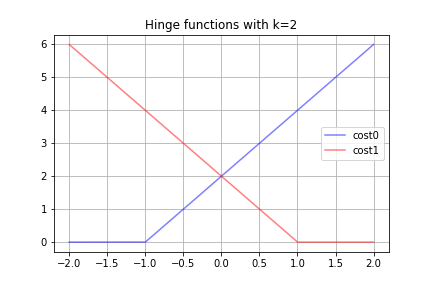
\includegraphics[scale=0.7]{hinge}
  \captionof{figure}{Graph of $cost_0$ and $cost_1$ with $k=2$}
  \label{fig:hinge}
\end{center}

\subsection{Projections}

Let be $E$ a vector space of dimension $n$. Let $F$ be a vector subspace  and $G$ a supplementary vector subspace to $F$ in $E$. As a reminder:

\begin{equation}
F \oplus G = E \iff F \cup G = E \text{ and } F \cap G = \{0\}
\end{equation}

Note that if $dim(F)<n$, then there is an infinite number of supplementary vector subspaces to $F$ in $E$. To get this point, consider the example of $\mathbb{R}^{2}$:

\begin{align*}
& F = Vect((1,1)) \\
& G_1 = Vect((2,1)) \text{ and } G_2 = Vect((0, 2)) \\
& G_1 \text{ and } G_2 \text{ are both supplementary subspaces to F for instance.}
\end{align*}

Given that $G$ is supplementary to $F$, we know that:

\begin{equation}
\forall x \in E, \exists! (a, b) \in F \times G \text{ such that } x = a +B
\end{equation}

We can define $p$ the linear application that gives the part $a$ of the decomposition of $x$. $p$ is a projection. Let focus on a special kind of projections called orthogonal projections. To do so, we will focus on the euclidean space $\mathbb{R}^{n}$ and we will take $F=Vect(y)$ where $y \in \mathbb{R}^{n}$. Now we will consider the supplementary vector subspace to $F$ that is orthogonal to it and we call it $G$. It is a vector subspace that verifies:

\begin{align*}
& \forall x \in G, <x, y> = 0 \\
& \text{ where } <. \: , .> \text{ is the scalar product operator} \\ 
& \text{i.e. } x^{\top}y = 0
\end{align*}

We can write that:

\begin{align*}
& \forall x \in \mathbb{R}^{n}, x = p(x) + x - p(x) \\
& \\
& \text{ where } p(x) \in Vect(y) \text{ and } x - p(x) \in G \\
& \\
& \text{ thus } \exists! k \in \mathbb{R}, p(x) = ky \text{ and } <x-p(x), y> = 0 \\
& \\
& \text{ replacing } p(x) \text{ in the second equation yields} \\
& \\
& k = \frac{<x, y>}{||y||^{2}} \\
& \\
& \text{ i.e. } p(x) = \frac{<x, y>}{||y||^{2}} * y \\
& \\
& \text{ where } ||x|| = \sqrt[2]{\sum_{i=1}^{m} x_{i}^{2}}
\end{align*}

\subsection{Large margin intuition}
 
Let go back to the SVM cost function. Assume that C is massively large, so much as we set the first term of the sum in the cost function $J(\theta)$ to be null. The minimization problem becomes:

\begin{align*}
& \min_{\theta} \theta^{\top}\theta \text{ subject to the constraints that } \\
& \\
& \text{ if } y^{i} = 1, {x^{(i)}}^{\top}\theta >= 1 \iff ||p(x)||*||\theta|| >= 1 \text{ based on previous section}
& \\
& \text{ if } y^{i} = 0, {x^{(i)}}^{\top}\theta <= -1 \iff  -||p(x)||*||\theta|| <= -1 \text{ based on previous section}
\end{align*} 

For the constraints to hold true, we need the length of the projections of both the positive and negative examples $x^{(i)}$ to be as large as possible. In other words, with a big C, minimizing the cost function is tantamount to finding the line spanned by $Vect(\theta)$ such that the orthogonal projections of both the positives examples and the negative examples on this line are the largest possible.

\section{Appendix}

aaa

\subsection{F-score}

aaa

\subsection{Vectorization tips}

aaa
\end{document}